\definecolor{ao}{rgb}{0.0, 0.0, 1.0}

\chapter{Caso de uso: Predicción de la próxima jornada}

En la figura \ref{fig:clas37} se muestra el ranking correspondiente a la jornada número 37 de la temporada 2014/2015 de la Liga BBVA. En este capítulo vamos a predecir los resultados y el ranking para la última jornada, la número 38, de la temporada 2014/2015 de la Liga BBVA haciendo uso de la aplicación.
\begin{figure}[H]
	\centering
	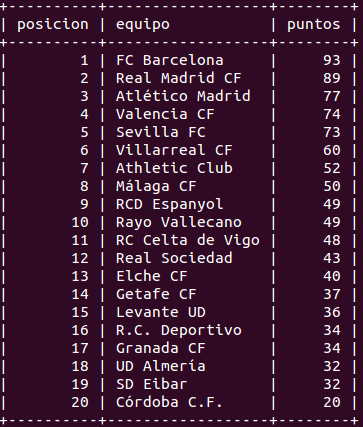
\includegraphics{images/cu1.png}
	\caption{Clasificación de la jornada 37.} \label{fig:clas37}
\end{figure}

 Los partidos que se disputarán en la jornada 38 son:
\begin{center}
	\begin{tabular}{|c|c|}
	\hline \rowcolor{ao} Local & Visitante \\ 
	\hline Levante UD & Elche CF \\ 
	\hline Athletic Club & Villarreal CF \\ 
	\hline FC Barcelona & R.C. Deportivo \\ 
	\hline Granada CF & Atlético de Madrid \\ 
	\hline Rayo Vallecano & Real Sociedad \\ 
	\hline SD Eibar & Córdoba C.F. \\ 
	\hline RC Celta de Vigo & RCD Espanyol \\ 
	\hline UD Almería & Valencia CF \\ 
	\hline Málaga CF & Sevilla FC \\ 
	\hline Real Madrid CF & Getafe CF \\ 
	\hline 
\end{tabular} 
\end{center}

Vamos a proceder a calcular las probabilidades de resultados de los partidos según los distintos modelos de predicción implementados.

\section{Modelo basado en la posición relativa}
Aplicando la interpolación lineal explicada en la sección 3.1. obtendremos las siguientes probabilidades para los partidos de la próxima jornada:
\begin{figure}[H]
	\centering
	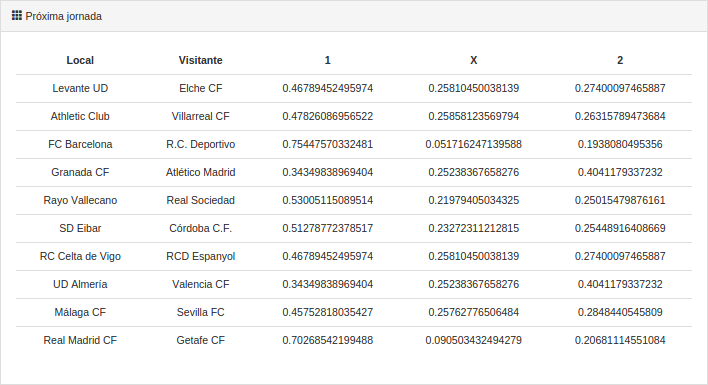
\includegraphics[scale=0.9]{images/cu2.png}
	\caption{Probabilidades usando el modelo basado en la posición relativa.} \label{fig:pred1}
\end{figure}

\newpage

En la siguiente figura se muestran los resultados finales de los partidos tras haberse disputado la jornada 38:
\begin{figure}[H]
	\centering
	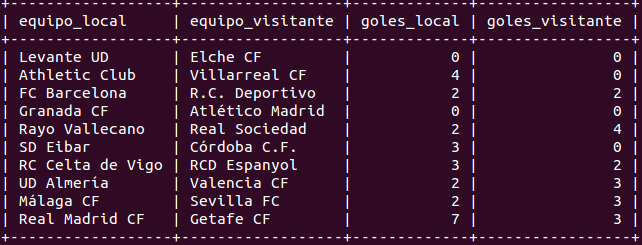
\includegraphics{images/cu3.png}
	\caption{Resultados de los partidos de la jornada 38.} \label{fig:result38}
\end{figure}
\ \\
Ahora vamos a analizar cuál sería el porcentaje de aciertos si comparamos los resultados de nuestra predicción (suponiendo que elegimos como resultado el que tenga mayor probabilidad) con los resultados reales una vez jugados los partidos.

\begin{center}
	\begin{tabular}{|c|c|c|c|c|}
		\hline \rowcolor{ao} Local & Visitante & Predicción & Resultado & Acierto \\ 
		\hline Levante UD & Elche CF & 1 & X & \begingroup\color{red}\xmark\endgroup \\ 
		\hline Athletic Club & Villarreal CF & 1 & 1 & \begingroup\color{green}\cmark\endgroup \\ 
		\hline FC Barcelona & R.C. Deportivo & 1 & X & \begingroup\color{red}\xmark\endgroup \\ 
		\hline Granada CF & Atlético de Madrid & 2 & X & \begingroup\color{red}\xmark\endgroup \\ 
		\hline Rayo Vallecano & Real Sociedad & 1 & 2 & \begingroup\color{red}\xmark\endgroup \\ 
		\hline SD Eibar & Córdoba C.F. & 1 & 1 & \begingroup\color{green}\cmark\endgroup \\ 
		\hline RC Celta de Vigo & RCD Espanyol & 1 & 1 & \begingroup\color{green}\cmark\endgroup \\ 
		\hline UD Almería & Valencia CF & 2 & 2 & \begingroup\color{green}\cmark\endgroup \\ 
		\hline Málaga CF & Sevilla FC & 1 & 2 & \begingroup\color{red}\xmark\endgroup \\ 
		\hline Real Madrid CF & Getafe CF & 1 & 1 & \begingroup\color{green}\cmark\endgroup \\ 
		\hline 
	\end{tabular} 
\end{center}

Acertamos 5 de los 10 enfrentamientos, es decir, la mitad de los partidos.\\

\newpage

Ahora procedemos a calcular el nuevo ranking usando los resultados anteriores, es decir, al ranking de la figura \ref{fig:clas37} le sumamos 3 puntos a cada equipos ganador y 1 a cada equipo que empata según nuestra predicción de la figura \ref{fig:pred1} obteniendo:\\


\begin{figure}[H]
	\centering
	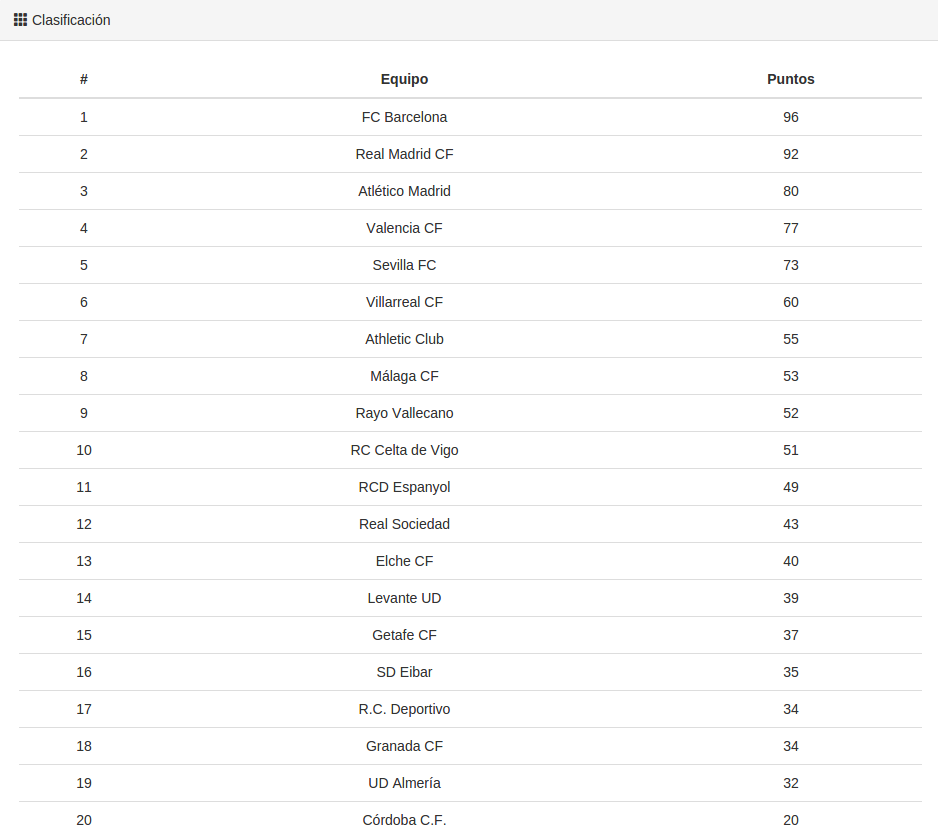
\includegraphics[scale=0.7]{images/cu4.png}
	\caption{Predicción de la clasificación usando el modelo basado en la posición relativa.} \label{fig:predclas1}
\end{figure}

\newpage
En la siguiente figura se muestra el ranking final tras disputarse la jornada 38:
\begin{figure}[H]
	\centering
	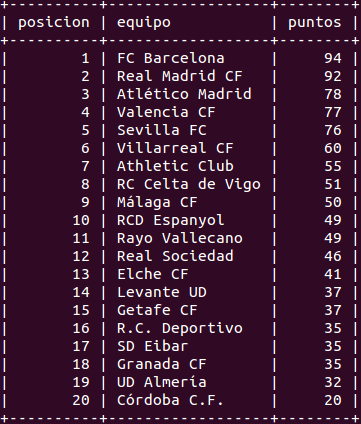
\includegraphics[scale=0.9]{images/cu5.png}
	\caption{Clasificación de la jornada 38.} \label{fig:clas38}
\end{figure}

Para realizar las comparaciones de rankings, disponemos de varios scripts que automatizan esta tarea. Tenemos tres maneras distintas de compararlos que veremos a continuación.\\

Vamos a proceder a comparar el ranking usando los resultados de la predicción (figura \ref{fig:predclas1}) y el ranking final al disputarse la jornada 38 (figura \ref{fig:clas38}): 
\begin{itemize}
	\item Si simplemente calculamos la tasa de aciertos comparando que los rankings coinciden posición por posición, un total de 14 de los 20 equipos estarían correctamente colocados, es decir, el porcentaje sería del $\dfrac{14}{20}=0.7$.  
	\item Si aplicamos la Rho de Spearman, explicada en la sección 2.2., obtenemos: $\psi = 0.82222$.
	\item Si aplicamos la Tau de Kendall, también explicada en la sección 2.2. de esta memoria, obtenemos: $\tau = 0.95789$.
\end{itemize}

Ahora tenemos que interpretar estos tres resultados. El porcentaje de aciertos coincidiendo posición a posición no nos es del todo útil, pues si hay poca diferencia de puntos entre varios equipos, no ``acertar'' el resultado de un solo equipo puede descolocar bastantes posiciones y ``penalizar'' significativamente el porcentaje de aciertos, por ello se suelen utilizar métodos de comparación de rankings como la Tau de Kendall y la Rho de Spearman. \\

El problema de la Rho de Spearman, que se basa en hallar la distancia entre las posiciones que ocupa el mismo equipo en los dos rankings, reside en que no es acotada, por lo que el análisis de esta medida tampoco nos va a ser de gran utilidad. \\

La medida que más información nos puede aportar en el estudio de la tasa de aciertos al comparar los dos rankings en cuestión es la Tau de Kendall. Esta medida analiza que la posición relativa para cada par de equipos (de los 190 pares totales) sea la misma en ambos rankings, superando el problema que surgía al hacer la comparación posición por posición. Cuanto más cercano a 1 sea el valor de la Tau de Kendall mayor será la cantidad de pares acertados y, por tanto, mejor será la tasa de aciertos. \\

En nuestro caso, el $0.95789$ de la Tau de Kendall se obtiene de $186$ pares concordantes y solo $4$ discordantes, por lo que la tasa de aciertos en el cálculo del ranking para la jornada 38 se puede considerar bastante buena a pesar de haber acertado tan solo el resultado de la mitad de los partidos.

\section{Modelo basado en la tendencia de cada equipo}
Vamos a calcular las probabilidades y clasificación para los mismos enfrentamientos de la jornada 38 usando las tres funciones memoria distintas propuestas en la sección 3.2.\\

Aplicando la función memoria constante (figura \ref{fig:constante}) obtenemos las siguientes probabilidades para los partidos:
\begin{figure}[H]
	\centering
	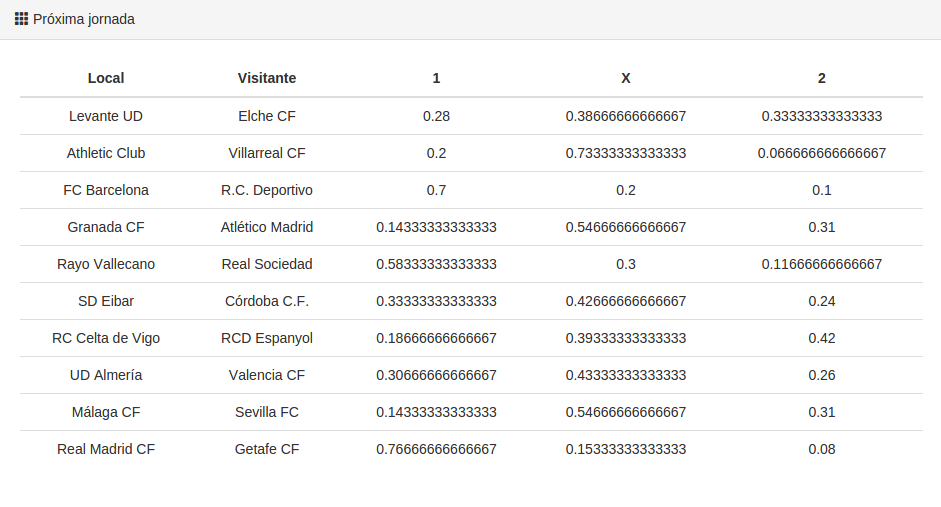
\includegraphics[scale=0.67]{images/cu6.png}
	\caption{Probabilidades usando la función memoria constante.}
\end{figure}

Aplicando la función memoria lineal (figura \ref{fig:lineal}) obtenemos las siguientes probabilidades:
\begin{figure}[H]
	\centering
	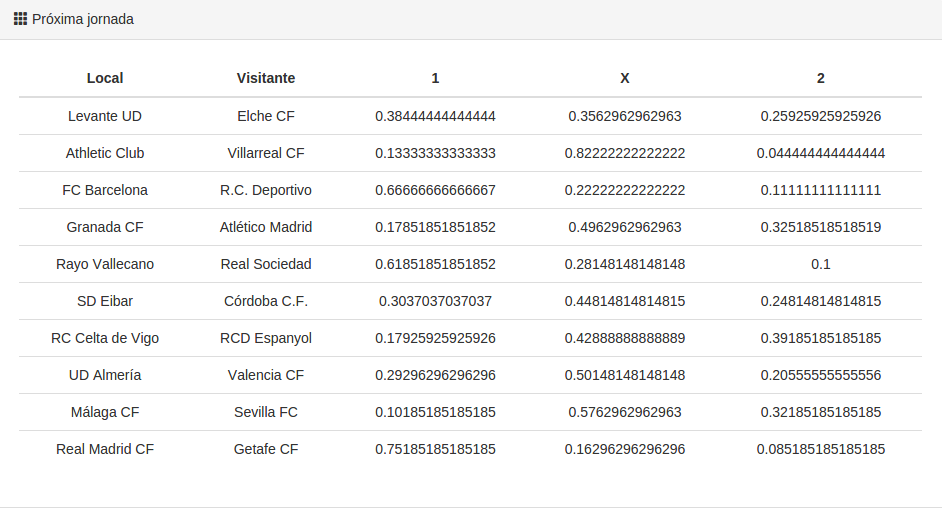
\includegraphics[scale=0.67]{images/cu7.png}
	\caption{Probabilidades usando la función memoria lineal.}
\end{figure}

Aplicando la función memoria exponencial (figura \ref{fig:exponencial}) obtenemos las siguientes probabilidades:
\begin{figure}[H]
	\centering
	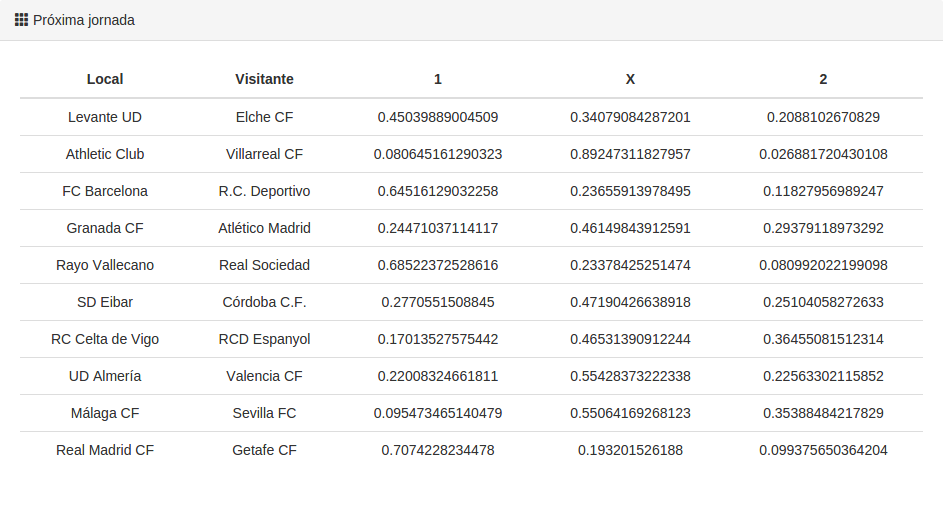
\includegraphics[scale=0.67]{images/cu8.png}
	\caption{Probabilidades usando la función memoria exponencial.}
\end{figure}

Ahora vamos a analizar cuál sería el porcentaje de aciertos si comparamos los resultados de nuestras predicciones (suponiendo que elegimos como resultado el que tenga mayor probabilidad) con los resultados reales una vez jugados los partidos (figura \ref{fig:result38}).

\begin{center}
	\begin{tabular}{|c|c|c|c|c|c|}
		\hline \rowcolor{ao} Local & Visitante & Constante & Lineal & Exponencial & Resultado \\ 
		\hline Levante UD & Elche CF & X & 1 & 1 & X \\ 
		\hline Athletic Club & Villarreal CF & X & X & X & 1 \\ 
		\hline FC Barcelona & R.C. Deportivo & 1 & 1 & 1 & X \\ 
		\hline Granada CF & Atlético de Madrid & X & X & X & X \\ 
		\hline Rayo Vallecano & Real Sociedad & 1 & 1 & 1 & 2\\ 
		\hline SD Eibar & Córdoba C.F. & X & X & X & 1\\ 
		\hline RC Celta de Vigo & RCD Espanyol & 2 & X & X & 1\\ 
		\hline UD Almería & Valencia CF & X & X & X & 2\\ 
		\hline Málaga CF & Sevilla FC & X & X & X & 2\\ 
		\hline Real Madrid CF & Getafe CF & 1 & 1 & 1 & 1\\ 
		\hline 
	\end{tabular} 
\end{center}
Usando la función constante acertamos 3 partidos, con la lineal 2 y con la exponencial 2, que del total de 10 jugados, da un porcentaje bastante malo. En este caso la predicción del modelo lineal y del exponencial son exactamente la misma, por tanto, se obtendrá el mismo ranking. A continuación se muestran los dos rankings resultantes:

\begin{figure}[H]
	\centering
	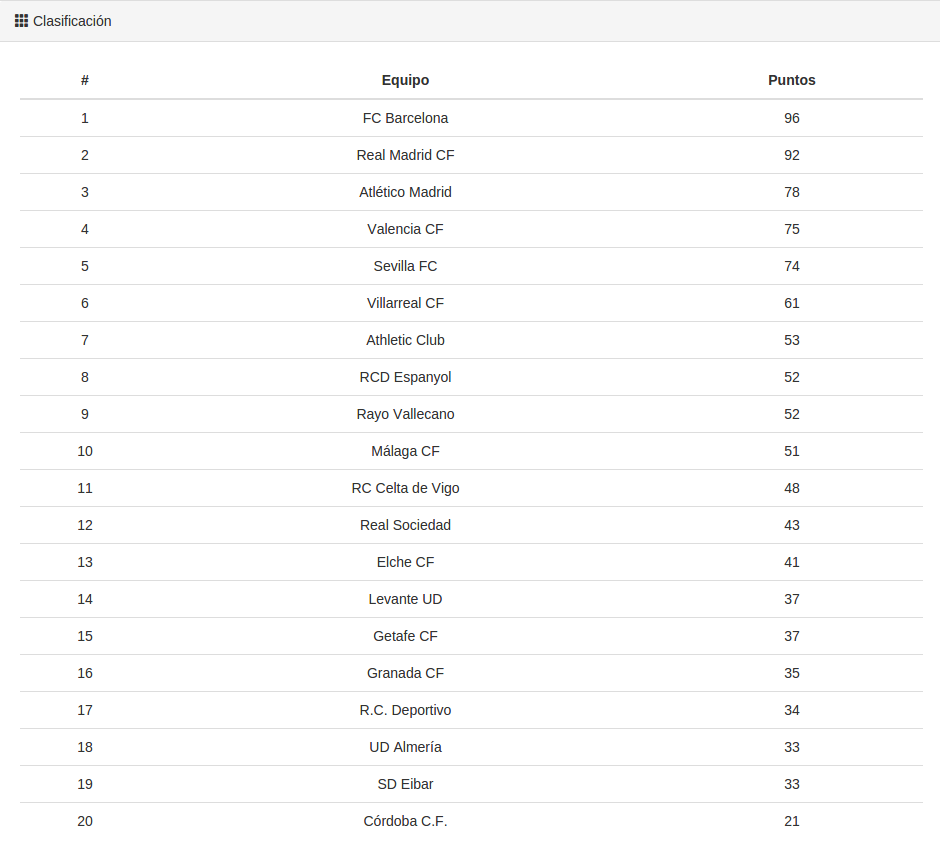
\includegraphics[scale=0.53]{images/cu9.png}
	\caption{Predicción de la clasificación usando la función constante.}
\end{figure}
\begin{figure}[H]
	\centering
	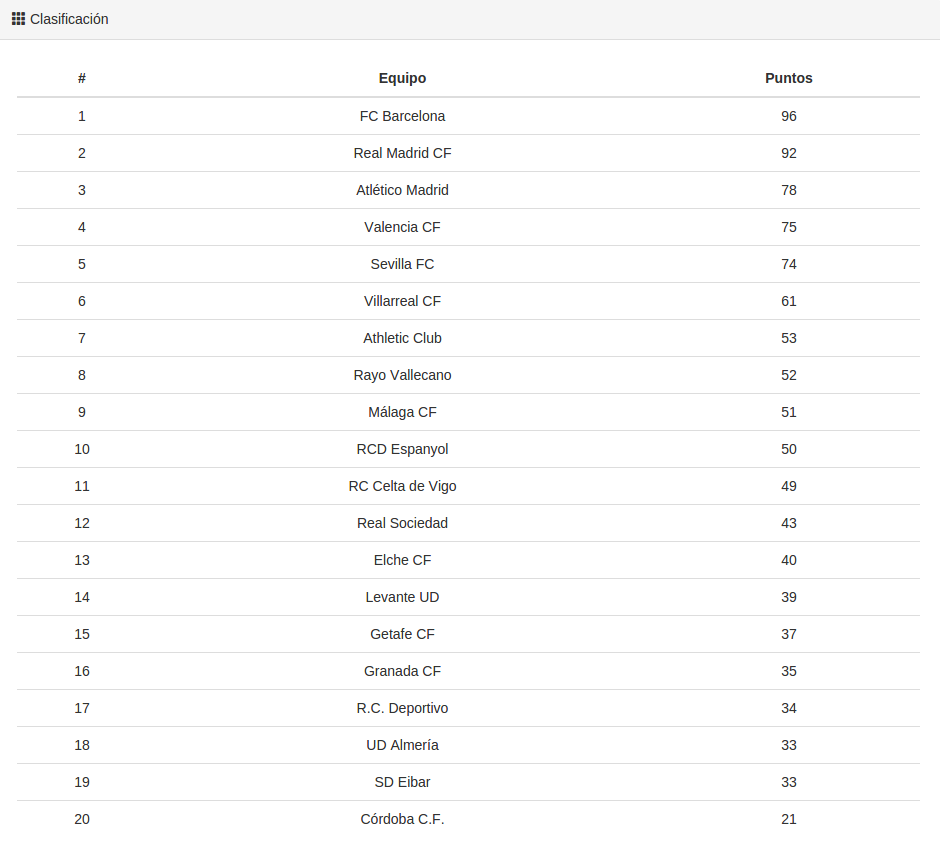
\includegraphics[scale=0.53]{images/cu10.png}
	\caption{Predicción de la clasificación usando las funciones lineal y exponencial.}
\end{figure}

Ahora calculamos la tasa de aciertos con el ranking de la figura \ref{fig:clas38} de las tres formas que explicamos en el modelo anterior.

\begin{center}
	\begin{tabular}{|c|c|c|}
	\hline  & F.M. Constante & F.M. Lineal/Exponencial \\ 
	\hline $\%$ posición por posición & 12 & 14 \\ 
	\hline Tau de Kendall ($\tau$) & 0.91578 & 0.91578 \\ 
	\hline Rho de Spearman ($\psi$) & 1.31903 & 1.11070 \\ 
	\hline 
\end{tabular} 
\end{center}

Como ya mencionamos, la medida de comparación de rankings más fiable es la Tau de Kendall, sin embargo, en este caso, es el mismo valor para las tres funciones memoria, con todos ellos se acertaría la posición relativa del mismo número de pares de equipos. Sin embargo, los otros dos valores nos indican que las funciones lineal y exponencial, a pesar de acertar un partido menos en la predicción de los resultados, tienen mejor porcentaje de aciertos al calcular la clasificación final.\\

Con este método, la predicción de resultados de partidos es bastante mala, aunque a la hora de predecir la clasificación obtenemos unos resultados aceptables, pero claramente inferiores a los obtenidos por el modelo basado en la posición de los equipos. 

\section{Combinación de los modelos}
El primer paso va a ser ejecutar un script que nos devuelve el valor de $\lambda$ con el que se obtiene el mayor número de aciertos entrenando sobre un histórico de datos, en este caso, entrenando sobre las jornadas que transcurren desde la 21 hasta la 37.\\

Tras un primer barrido (recorrer de $\lambda=0$ hasta $\lambda=1$ con paso $0.1$), obtenemos que el mayor porcentaje de aciertos se concentra en torno al $\lambda=0.8$. Ahora hacemos un refinamiento estudiando los valores de $\lambda$ entre $0.7$ y $0.9$ aumentando cada vez $0.01$. El resultado es que el mayor número de aciertos que se obtiene es un total de 92 (de 170 enfrentamientos) cuando $\lambda \in [0.73,0.80]$. Elegimos un valor de dicho intervalo, por ejemplo, $\lambda=0.80$ y lo fijamos. \\
Recordemos que el primer modelo propuesto tenía mayor porcentaje de aciertos que el segundo, por lo que es lógico que el valor de $\lambda$ esté inclinado a dar más ``peso'' al primero que al segundo. \\

Aplicando la combinación convexa con $\lambda=0.8$ obtenemos los siguientes porcentajes para los enfrentamientos de la jornada 38:

\begin{figure}[H]
	\centering
	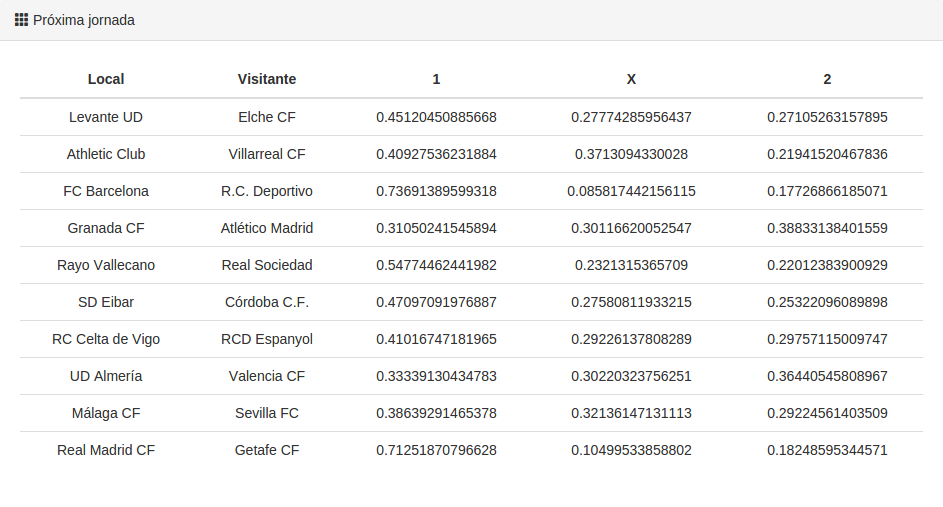
\includegraphics[scale=0.7]{images/cu11.png}
	\caption{Probabilidades usando la combinación convexa de los modelos.}
\end{figure}

Ahora vamos a analizar cuál sería el porcentaje de aciertos si comparamos los resultados de nuestra predicción (suponiendo que elegimos como resultado el que tenga mayor probabilidad) con los resultados reales una vez jugados los partidos (figura \ref{fig:result38}).

\begin{center}
	\begin{tabular}{|c|c|c|c|c|}
		\hline \rowcolor{ao} Local & Visitante & Predicción & Resultado & Acierto \\ 
		\hline Levante UD & Elche CF & 1 & X & \begingroup\color{red}\xmark\endgroup \\ 
		\hline Athletic Club & Villarreal CF & 1 & 1 & \begingroup\color{green}\cmark\endgroup \\ 
		\hline FC Barcelona & R.C. Deportivo & 1 & X & \begingroup\color{red}\xmark\endgroup \\ 
		\hline Granada CF & Atlético de Madrid & 2 & X & \begingroup\color{red}\xmark\endgroup \\ 
		\hline Rayo Vallecano & Real Sociedad & 1 & 2 & \begingroup\color{red}\xmark\endgroup \\ 
		\hline SD Eibar & Córdoba C.F. & 1 & 1 & \begingroup\color{green}\cmark\endgroup \\ 
		\hline RC Celta de Vigo & RCD Espanyol & 1 & 1 & \begingroup\color{green}\cmark\endgroup \\ 
		\hline UD Almería & Valencia CF & 2 & 2 & \begingroup\color{green}\cmark\endgroup \\ 
		\hline Málaga CF & Sevilla FC & 1 & 2 & \begingroup\color{red}\xmark\endgroup \\ 
		\hline Real Madrid CF & Getafe CF & 1 & 1 & \begingroup\color{green}\cmark\endgroup \\ 
		\hline 
	\end{tabular} 
\end{center}

En este caso en concreto, los resultados son los mismos que los que obtuvimos aplicando el modelo basado en la posición relativa de los equipos, por lo que el ranking obtenido será el mismo que el que obtuvimos en la figura \ref{fig:predclas1} y los valores obtenidos al compararlo con el ranking final (figura \ref{fig:clas38}) también coincidirán.\\

\section{Resultados}
Aplicando los distintos modelos a la jornada 38 de la temporada 2014/2015, hemos sacado las siguientes conclusiones:
\begin{itemize}
	\item El modelo basado en la tendencia de los equipos es inferior a los otros dos modelos propuestos.
	\item En este caso, con el modelo basado en la posición relativa de los equipos y con la combinación de modelos se obtienen exactamente los mismos resultados. En el siguiente capítulo haremos un estudio más extenso que demostrará que el modelo combinatorio será el que tendrá mayor tasa de acierto.
	\item El porcentaje de aciertos en los resultados de los partidos no nos va a servir para hacernos millonarios echando la Quiniela, sin embargo, es un porcentaje aceptable (un $50\%$ de aciertos usando el primer y tercer modelo) superiores a métodos como el de selección aleatoria ($33 \%$) o el método de elección de victoria local (en este caso sería de un $40\%$).
	\item Pero la tasa de aciertos aumenta considerablemente cuando comparamos el ranking calculado usando la predicción con el ranking al final de la jornada. La Tau de Kendall que nos indica el porcentaje de pares de equipos que tienen la misma posición relativa (en ambos el equipo A aparece por encima del equipo B o en ambos el equipo B aparece por encima del equipo A) aplicando nuestros modelos se encuentra por encima del $90\%$.
\end{itemize}
 
